\section{moeo\-Aggregative\-Comparator$<$ MOEOT $>$ Class Template Reference}
\label{classmoeoAggregativeComparator}\index{moeoAggregativeComparator@{moeoAggregativeComparator}}
Functor allowing to compare two solutions according to their fitness and diversity values, each according to its aggregative value.  


{\tt \#include $<$moeo\-Aggregative\-Comparator.h$>$}

Inheritance diagram for moeo\-Aggregative\-Comparator$<$ MOEOT $>$::\begin{figure}[H]
\begin{center}
\leavevmode
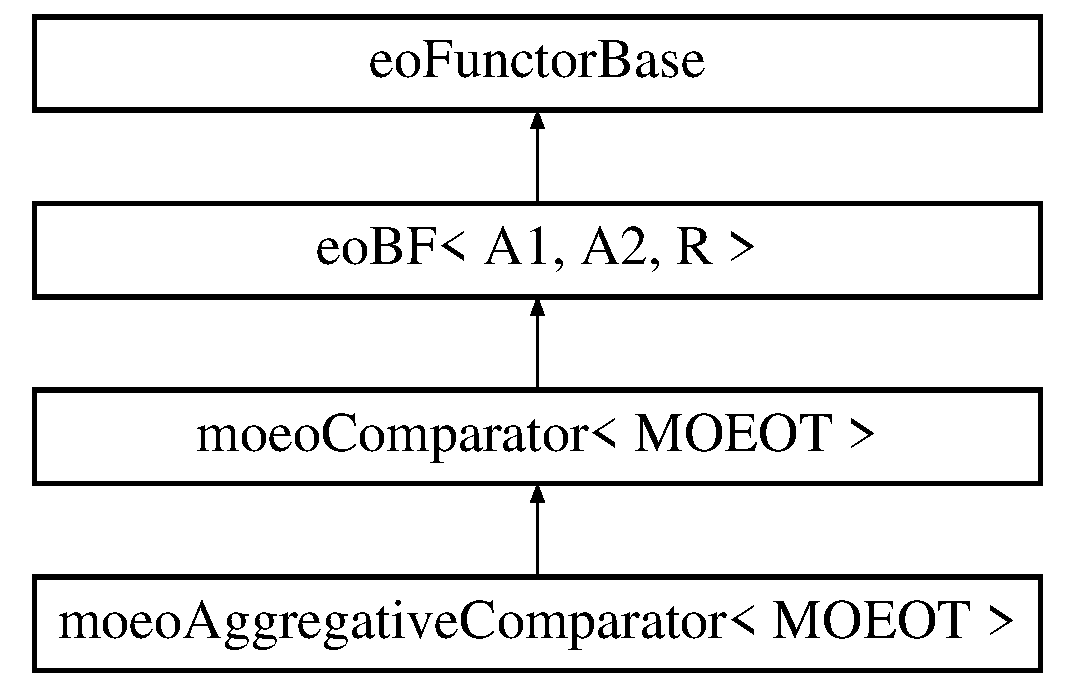
\includegraphics[height=4cm]{classmoeoAggregativeComparator}
\end{center}
\end{figure}
\subsection*{Public Member Functions}
\begin{CompactItemize}
\item 
\bf{moeo\-Aggregative\-Comparator} (double \_\-weight\-Fitness=1.0, double \_\-weight\-Diversity=1.0)
\begin{CompactList}\small\item\em Ctor. \item\end{CompactList}\item 
const bool \bf{operator()} (const MOEOT \&\_\-moeo1, const MOEOT \&\_\-moeo2)
\begin{CompactList}\small\item\em Returns true if \_\-moeo1 $<$ \_\-moeo2 according to the aggregation of their fitness and diversity values. \item\end{CompactList}\end{CompactItemize}
\subsection*{Private Attributes}
\begin{CompactItemize}
\item 
double \bf{weight\-Fitness}\label{classmoeoAggregativeComparator_9ddf44b9e447bee8503c5b9cad9a7df0}

\begin{CompactList}\small\item\em the weight for fitness \item\end{CompactList}\item 
double \bf{weight\-Diversity}\label{classmoeoAggregativeComparator_d4ce25f797af0218c6c8cfca7c73b2d3}

\begin{CompactList}\small\item\em the weight for diversity \item\end{CompactList}\end{CompactItemize}


\subsection{Detailed Description}
\subsubsection*{template$<$class MOEOT$>$ class moeo\-Aggregative\-Comparator$<$ MOEOT $>$}

Functor allowing to compare two solutions according to their fitness and diversity values, each according to its aggregative value. 



Definition at line 45 of file moeo\-Aggregative\-Comparator.h.

\subsection{Constructor \& Destructor Documentation}
\index{moeoAggregativeComparator@{moeo\-Aggregative\-Comparator}!moeoAggregativeComparator@{moeoAggregativeComparator}}
\index{moeoAggregativeComparator@{moeoAggregativeComparator}!moeoAggregativeComparator@{moeo\-Aggregative\-Comparator}}
\subsubsection{\setlength{\rightskip}{0pt plus 5cm}template$<$class MOEOT$>$ \bf{moeo\-Aggregative\-Comparator}$<$ MOEOT $>$::\bf{moeo\-Aggregative\-Comparator} (double {\em \_\-weight\-Fitness} = {\tt 1.0}, double {\em \_\-weight\-Diversity} = {\tt 1.0})\hspace{0.3cm}{\tt  [inline]}}\label{classmoeoAggregativeComparator_76cc4d0f5f9bd4984c77410ad8142914}


Ctor. 

\begin{Desc}
\item[Parameters:]
\begin{description}
\item[{\em \_\-weight\-Fitness}]the weight for fitness \item[{\em \_\-weight\-Diversity}]the weight for diversity \end{description}
\end{Desc}


Definition at line 54 of file moeo\-Aggregative\-Comparator.h.

\subsection{Member Function Documentation}
\index{moeoAggregativeComparator@{moeo\-Aggregative\-Comparator}!operator()@{operator()}}
\index{operator()@{operator()}!moeoAggregativeComparator@{moeo\-Aggregative\-Comparator}}
\subsubsection{\setlength{\rightskip}{0pt plus 5cm}template$<$class MOEOT$>$ const bool \bf{moeo\-Aggregative\-Comparator}$<$ MOEOT $>$::operator() (const MOEOT \& {\em \_\-moeo1}, const MOEOT \& {\em \_\-moeo2})\hspace{0.3cm}{\tt  [inline]}}\label{classmoeoAggregativeComparator_2f6745ebc2d575e64b162fc250f04b0f}


Returns true if \_\-moeo1 $<$ \_\-moeo2 according to the aggregation of their fitness and diversity values. 

\begin{Desc}
\item[Parameters:]
\begin{description}
\item[{\em \_\-moeo1}]the first solution \item[{\em \_\-moeo2}]the second solution \end{description}
\end{Desc}


Definition at line 63 of file moeo\-Aggregative\-Comparator.h.

References moeo\-Aggregative\-Comparator$<$ MOEOT $>$::weight\-Diversity, and moeo\-Aggregative\-Comparator$<$ MOEOT $>$::weight\-Fitness.

The documentation for this class was generated from the following file:\begin{CompactItemize}
\item 
moeo\-Aggregative\-Comparator.h\end{CompactItemize}
